\chapter{Singular Perturbation} \label{chap:singular-perturbation}
This chapter is dedicated to analyze the polynomial eigenvalue problem with transonic velocity profiles. We will first show the existence of the singularity of Eq.(\ref{eq:polynomial-eigenvalue-problem}), then we will discuss the concept of singular perturbation and the way we solve the problem.

\section{Presence of Singularity in Transonic cases} \label{sec:presence-of-singularity}
In order to see the existence of the singularity, we rearrange the terms the polynomial eigenvalue problem, Eq.(\ref{eq:polynomial-eigenvalue-problem}),
\begin{equation} \label{eq:singular-perturbation-problem}
	\begin{aligned}
		  & (1-v_0^2)\pdv[2]{\tilde{v}}{z}                                                                                                                                        \\
		+ & \left[2i\omega v_0 - \left(3v_0 + \frac{1}{v_0}\right)\pdv{v_0}{z}\right]\pdv{\tilde{v}}{z}                                                                           \\
		+ & \left[\omega^2 + 2i\omega\pdv{v_0}{z} -\left(1 - \frac{1}{v_0^2}\right)\left(\pdv{v_0}{z}\right)^2 - \left(v_0 + \frac{1}{v_0}\right)\pdv[2]{v_0}{z} \right]\tilde{v} \\
		= & 0
	\end{aligned}
\end{equation}
This is a second order ordinary differential equation defined on region $[-1,1]$.

For transonic (accelerating and decelerating) velocity profiles (Fig.\ref{fig:velocity-profiles}), the plasma flow is at sonic point at the throat of the nozzle, $v_0(0)=1$. Therefore, the highest order term vanishes at $z=0$. This causes the failure of spectral method, see Fig.(\ref{chap:discussion}). It can be proved that $z=0$ is a regular singular point.

\begin{figure} [htbp]
	\centering
	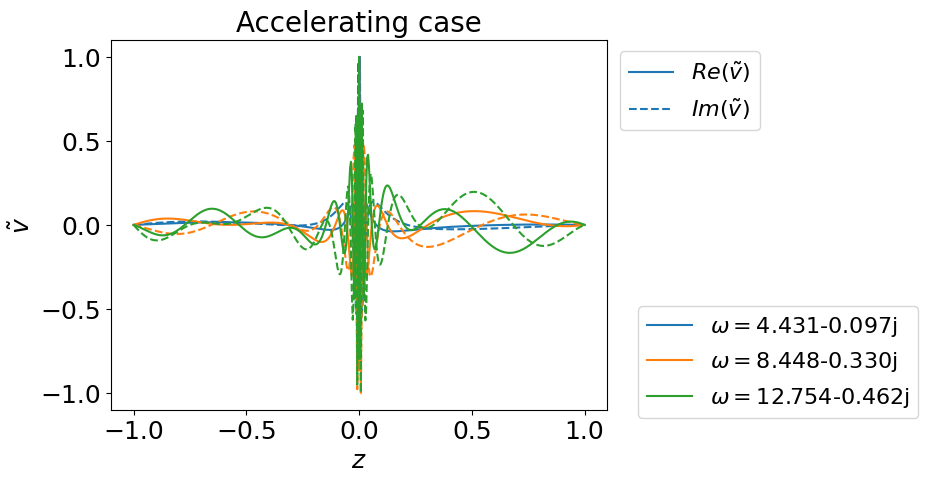
\includegraphics[width=0.7\textwidth]{figures/results-bad-accelerating-v}
	\caption{An attempt to solve the polynomial eigenvalue problem, Eq.(\ref{eq:polynomial-eigenvalue-problem}) using finite-difference. Eigenfunctions are squeezed to the center of the nozzle due to the existence of the singularity at $z=0$.}
	\label{fig:failure-of-spectral-method}
\end{figure}

\section{Connection of Transonic fluid Flow to Black Hole}
Consider a transonic fluid flow, the sound waves can propagate from the subsonic region into the supersonic region, while propagating in the opposite direction is not allowed. This process is similar to masses falling into the black hole. Therefore, the sonic point of a transonic flow is an acoustic equivalent of event horizon of a black hole. Hence, a transonic flow is sometimes called an acoustic black hole. \cite{okuzumi_sakagami_quasinormal_2007}

\subsection{The Schr{\"o}dinger-Type Wave Equation}
In de Labal nozzle, the governing equations for quasi-one-dimensional flow of a perfect fluid are
\begin{align}
	\pdv{\rho A}{t}	+ \pdv{\rho vA}{z} & = 0            \label{eq:fluid-continuity} \\
	\rho\pdv{v}{t}	+ \rho\pdv{v}{z}    & = -\pdv{p}{z}  \label{eq:fluid-momentum}   \\
	p                                  & = \rho^\gamma \label{eq:fluid-energy}
\end{align}
where $\rho$ is the density, $v$ is the velocity, $p$ is the pressure, $A$ is the cross section of the nozzle, and $\gamma=1.4$ is the heat capacity ratio for air. The governing equations, Eq.(\ref{eq:fluid-continuity}), (\ref{eq:fluid-momentum}), and (\ref{eq:fluid-energy}) above are conservation of density, momentum and energy, respectively.

We can reduce Eq.(\ref{eq:fluid-momentum}) to Bernoulli's equation
\begin{equation} \label{eq:bernoulli}
	\pdv{\Phi}{t} + \frac{1}{2}\left(\pdv{\Phi}{z}\right)^2 + h(\rho) = 0
\end{equation}
where $h(\rho)=\int \rho^{-1}dp$ is the specific enthalpy and $\Phi=\int vdz$ is the velocity potential.

Now, we introduce the acoustic analogy of tortoise coordinate and a new function $H_\omega(z)$,
\[ z^* = c_{s0} \int \frac{dz}{c_s(1-M^2)} \]
\[ H_\omega(z) = g^{1/2} \int dt e^{i\omega [t-f(z)]} \phi(t,x) \]
where $c_s = \sqrt{\gamma p/\rho}$, $c_{s0}$ is the stagnation sound speed, it is a constant over isentropic region, $M = v/c_s$ is the Mach number, $g=\rho A/c_s$ and
\[ f(x) = \int \frac{\abs{v} dz}{c_s^2 - v^2} \]

If we perturb the density and the velocity potential by $\delta\rho$ and $\phi$, respectively. Then employ the acoustic analogy of tortoise coordinate, the linearized wave equation for sounds can be transformed to a Schr{\"o}dinger-type wave equation,
\[ \left[\dv[2]{{z^*}} + \kappa^2 - V(z^*)\right] H_{\omega} = 0 \]
where $\omega$ is the oscillating frequency of the perturbation, $\kappa = \omega/c_{s0}$ is the normalized frequency, and the effective potential
\[ V(z^*) = \frac{1}{g^2} \left[ \frac{g}{2}\dv[2]{g}{{z^*}} - \frac{1}{4}\left(\dv{g}{z^*}\right)^2 \right] \]
The effective potential $V(z^*)$ has dimension of $(\text{length})^{-2}$ and characterizes the "curvature scattering" of sound waves on the acoustic black hole. \cite{okuzumi_sakagami_quasinormal_2007} By employing the acoustic tortoise coordinate, the singularity at the sonic point is pushed to infinity. When doing numerical simulations, we can solve the Schr{\"o}dinger-type equation separately in subsonic and supersonic region of the nozzle.

It turns out, scalar field perturbations in the minimally geometric deformed brane-world black hole background yields a very similar wave-like equation, \cite{da_rocha_black_2017}
\[ \left[ \dv[2]{{r^*}} + \omega^2 - V(r^*) \right] \Psi(r^*) = 0 \]
where $r^*$ is the tortoise coordinate.

\section{Singular Perturbation Problem}
In the previous section, we introduced transonic fluid flow as an acoustic analogy of black hole and transformed the Eq.\ref{eq:bernoulli} to a Schr{\"o}dinger-type wave equation. This is an overkill for our problem. In this section, we will introduce a simpler way to deal with the singularity.

Consider Eq.(\ref{eq:polynomial-eigenvalue-problem}) as a boundary value problem by fixing the value of $\omega$,
The boundary value problem Eq.(\ref{eq:singular-perturbation-problem}) is defined on region $[-1,1]$, but the boundary values are defined on $z=-1$ and $z=0$. This is because to extract a regular solution near the singularity, we need to assume the solution is finite at the throat of the nozzle, $z=0$. This condition serves as a boundary value to the problem. Together with the boundary condition at the entrance of the nozzle, $\tilde{v}(-1) = 0$, the solutions to the boundary value problem, Eq.(\ref{eq:singular-perturbation-problem}) is fully determined up to a set of eigenvalues.

As we discuss in the earlier section, Sec.\ref{sec:presence-of-singularity}, $(1-v_0^2)$ is 0 at the nozzle throat $z=0$ since $v_0(z)$ is now a transonic velocity profile. This makes the problem a first order ordinary differential equation,
\[
	\left( 2i\omega - 4\eval{\pdv{v_0}{z}}_{z=0} \right)\pdv{\tilde{v}}{z}
	+ \left[2i\omega\eval{\pdv{v_0}{z}}_{z=0} - 2\eval{\pdv[2]{v_0}{z}}_{z=0} \right]\tilde{v}  = 0
\]
It is clear that the solution to this first order ODE has a totally different characteristics than the solution in the neighborhood of $z=0$. That means we cannot simply set $(1-v_0^2)$ to 0 and get an asymptotic approximation to the solution of Eq.(\ref{eq:singular-perturbation-problem}) near $z=0$. This is exactly the characteristics of singular perturbation problem.

\section{Expansion at Singularity}
The singularity is a regular singular point, we are able to extract finite solution near the singularity. In order to do so, we need to expand terms in Eq.(\ref{eq:singular-perturbation-problem}) about the singularity.

The first task is to linearize the terms with $v_0$ about the singularity. The linearization of $v_0(z) = 1 + v_0'(0)z$ is a good approximation to the original function $v_0(z)$ because the transonic velocity profiles are straight in the neighborhood of $z=0$, as we can see from Fig.\ref{fig:velocity-profiles}. Therefore, through some simple algebra we obtain,
\begin{equation}
	\begin{aligned}
		1-v_0^2              & = -2v_0'(0)z    \\
		3v_0 + \frac{1}{v_0} & = 4 + 2v_0'(0)z \\
		1-\frac{1}{v_0^2}    & = 2v_0'(0)z     \\
		v_0 + \frac{1}{v_0}  & = 2
	\end{aligned}
\end{equation}

Then Eq.(\ref{eq:singular-perturbation-problem}) becomes
\begin{equation} \label{eq:perturbed-equation-full}
	\begin{aligned}
		- & 2v_0'(0)z\pdv[2]{\tilde{v}}{z}                                              \\
		+ & [2i\omega - 4v_0'(0) + (2i\omega - 2v_0'(0))z]\pdv{\tilde{v}}{z}            \\
		+ & \left[\omega^2 + 2i\omega v_0'(0) - 2v_0''(0) - 2v_0'(0)^3z\right]\tilde{v}
		= 0
	\end{aligned}
\end{equation}

In fact, we can further simply the equation by dropping all $z$ terms except the first term (second-order derivative term). It can be shown that dropping the $z$ terms in Eq.(\ref{eq:perturbed-equation-full}) does not affect the first order correction ($\tilde{v}$ is the same up to $z$ term), it is an acceptable approximation.

\[ - 2v_0'(0)z\pdv[2]{\tilde{v}}{z}
	+ (2i\omega - 4v_0'(0))\pdv{\tilde{v}}{z}
	+ (\omega^2 + 2i\omega v_0'(0) - 2v_0''(0))\tilde{v}
	= 0 \]

Dividing by the first coefficient, we have
\begin{equation}
	z\pdv[2]{\tilde{v}}{z} + a\pdv{\tilde{v}}{z} + b\tilde{v} = 0
	\label{eq:perturbed-equation}
\end{equation}
where
\[ a = \frac{2i\omega - 4v_0'(0)}{-2v_0'(0)}; \quad
	b = \frac{\omega^2 + 2i\omega v_0'(0) - 2v_0''(0)}{-2v_0'(0)}
\]

Use Frobenius method, we assume the velocity perturbation can be written as a power series in $z$,  $\tilde{v} = \sum_{n\geq 0}c_nz^{n+r}$. By substituting the power series into Eq.(\ref{eq:perturbed-equation}) we have
\[ \sum_{n \geq 0} (n+r)(n+r+1) c_n z^{n+r-1} + a(n+r)c_nz^{n+r-1} + bc_nz^{n+r} = 0\]
Shift the power of the last term we get
\[ \sum_{n \geq 0} (n+r)(n+r+1) c_n z^{n+r-1} + a(n+r)c_nz^{n+r-1} + \sum_{n \geq 1} bc_{n-1}z^{n+r-1} = 0\]

Setting $n=0$, we get the indicial equation
\[ c_0 r(r-1) + c_0 ar = 0 \Rightarrow c_0r(r+a-1) = 0 \]
We get two different roots, $r=0$ and $r=1-a$. They correspond to finite solution and diverging solution near the singularity, respectively.

The coefficients are given by recurrence relation
\[ (n+r)(n+r-1)c_n + a(n+r)c_n + bc_{n-1} = 0
	\Rightarrow
	c_n = \frac{-bc_{n-1}}{(n+r)(n+r-1+a)}
\]
Solving this relation we get explicit expression for $c_n$, $n\in\mathbb{N}$,
\begin{equation}
	\begin{aligned}
		c_n & = \frac{(-1)^n b^n c_0}{\prod_{k=0}^{n-1} (n+r-k)(n+r-1+a-k)}              \\
		    & = (-1)^n b^n c_0 \frac{\Gamma(r+1)\Gamma(r+a)}{\Gamma(n+r+1)\Gamma(n+r+a)}
	\end{aligned}
	\label{eq:coefficient}
\end{equation}

Therefore, we successfully extracted the regular solution (corresponding to the root $r=0$) in the form of power series,
\begin{equation} \label{eq:regular-solution}
	\begin{aligned}
		\tilde{v} & = c_0 + c_1z + c_2z^2 + \cdots                               \\
		          & = c_0 - c_0\frac{b}{a}z + c_0\frac{b^2}{2a(1+a)}z^2 + \cdots
	\end{aligned}
\end{equation}

It is worth to mention that the diverging solution (corresponding to the root $r=a$) goes like
\[ \tilde{v}(z) \sim z^{1-a} = z^{-1-\omega_i/v_0'(0)}z^{i\omega_r/v_0'(0)}  \]
where $\omega = \omega_r + i\omega_i$. Meaning that the divergent solution will start to diverge when $\omega_i > -v'(0)$.

\section{Shooting Method}
Shooting method can be used to solve eigenvalue problem with specified boundary values,
\begin{equation} \label{eq:boundary-eigenvalue-problem}
	g(\tilde{v}(z);\omega) = 0,
	\quad
	z_l \leq z \leq z_r,
	\quad
	\tilde{v}(z_l) = \tilde{v}_l, \tilde{v}(z_r) = \tilde{v}_r
\end{equation}
where $\omega$ is the eigenvalue to be solved.

Suppose an eigenvalue problem can be formulated as
\[ \dv{z}\mathbf{u} = \mathbf{f}(\mathbf{u},z;\omega),
	\quad
	z_l<z<z_r,
	\quad
	\mathbf{u}(z_l) = \mathbf{u}_l
\]
where $\mathbf{u}\in\mathbb{R}^2$. Fixed an $\omega$, we can approximate $\mathbf{u}(z_r)$ by applying algorithms such as Runge-Kutta or Leap-frog.

Define $F$ by $F(\mathbf{u}_l;\omega)=\tilde{v}(z_r;\omega)$. This function $F$ takes in the initial value $\mathbf{u}_l$ and a fixed $\omega$, and outputs the "landing point" $\tilde{v}(z_r;\omega)$. If $\omega$ is an eigenvalue of Eq.(\ref{eq:boundary-eigenvalue-problem}), then $\tilde{v}(z_r;\omega) = \tilde{v}_r$. Now we can find eigenvalues to Eq.(\ref{eq:boundary-eigenvalue-problem}) by solving the roots to the scalar equation
\[h(\omega) = F(\mathbf{u}_l;\omega) - \tilde{v}_r\]

Having this higher view of shooting method in mind, we first transform Eq.(\ref{eq:polynomial-eigenvalue-problem}) to a IVP,
\begin{align*}
	v' & = u                        \\
	u' & = \frac{-1}{1-v_0^2}\left[
		\omega^2v + 2i\omega(v_0+v_0'v) - \left(3v_0 - \frac{1}{v_0}\right)v_0'u - \left(1-\frac{1}{v_0}^2\right)(v_0')^2v - \left(v_0+\frac{1}{v_0}v_0'' v\right)
		\right]
\end{align*}
and $v(0)=c_0=1,u(0)=c_1=(2i\omega v_0'-2v_0'')/2v_0'$. Moreover, $u'(0)=c_2=-((v_0')^4+(2i\omega v_0' + (v_0')^2 - v_0'')(i\omega v_0' - v_0''))/(v_0'(2i\omega-6v_0'))$.

In order to get initially value for cases with transonic velocity profiles, we need to expand the solution at the singularity.

